\documentclass{article}\usepackage[]{graphicx}\usepackage[]{color}
% maxwidth is the original width if it is less than linewidth
% otherwise use linewidth (to make sure the graphics do not exceed the margin)
\makeatletter
\def\maxwidth{ %
  \ifdim\Gin@nat@width>\linewidth
    \linewidth
  \else
    \Gin@nat@width
  \fi
}
\makeatother

\definecolor{fgcolor}{rgb}{0.345, 0.345, 0.345}
\newcommand{\hlnum}[1]{\textcolor[rgb]{0.686,0.059,0.569}{#1}}%
\newcommand{\hlstr}[1]{\textcolor[rgb]{0.192,0.494,0.8}{#1}}%
\newcommand{\hlcom}[1]{\textcolor[rgb]{0.678,0.584,0.686}{\textit{#1}}}%
\newcommand{\hlopt}[1]{\textcolor[rgb]{0,0,0}{#1}}%
\newcommand{\hlstd}[1]{\textcolor[rgb]{0.345,0.345,0.345}{#1}}%
\newcommand{\hlkwa}[1]{\textcolor[rgb]{0.161,0.373,0.58}{\textbf{#1}}}%
\newcommand{\hlkwb}[1]{\textcolor[rgb]{0.69,0.353,0.396}{#1}}%
\newcommand{\hlkwc}[1]{\textcolor[rgb]{0.333,0.667,0.333}{#1}}%
\newcommand{\hlkwd}[1]{\textcolor[rgb]{0.737,0.353,0.396}{\textbf{#1}}}%
\let\hlipl\hlkwb

\usepackage{framed}
\makeatletter
\newenvironment{kframe}{%
 \def\at@end@of@kframe{}%
 \ifinner\ifhmode%
  \def\at@end@of@kframe{\end{minipage}}%
  \begin{minipage}{\columnwidth}%
 \fi\fi%
 \def\FrameCommand##1{\hskip\@totalleftmargin \hskip-\fboxsep
 \colorbox{shadecolor}{##1}\hskip-\fboxsep
     % There is no \\@totalrightmargin, so:
     \hskip-\linewidth \hskip-\@totalleftmargin \hskip\columnwidth}%
 \MakeFramed {\advance\hsize-\width
   \@totalleftmargin\z@ \linewidth\hsize
   \@setminipage}}%
 {\par\unskip\endMakeFramed%
 \at@end@of@kframe}
\makeatother

\definecolor{shadecolor}{rgb}{.97, .97, .97}
\definecolor{messagecolor}{rgb}{0, 0, 0}
\definecolor{warningcolor}{rgb}{1, 0, 1}
\definecolor{errorcolor}{rgb}{1, 0, 0}
\newenvironment{knitrout}{}{} % an empty environment to be redefined in TeX

\usepackage{alltt}

\usepackage{authblk}


\title{Test}
\author{Huvinesh Rajendran (0340325)}

\affil{Bachelor of Computer Science}

\date{08-10-2021}
\IfFileExists{upquote.sty}{\usepackage{upquote}}{}
\begin{document}
\maketitle{}


\section{Question 1}
Explore and understand the R built-in mtcars data set.\\


\textbf{Answer}\\
\begin{knitrout}
\definecolor{shadecolor}{rgb}{0.969, 0.969, 0.969}\color{fgcolor}\begin{kframe}
\begin{alltt}
\hlkwd{str}\hlstd{(mtcars)}
\end{alltt}
\begin{verbatim}
## 'data.frame':	32 obs. of  11 variables:
##  $ mpg : num  21 21 22.8 21.4 18.7 18.1 14.3 24.4 22.8 19.2 ...
##  $ cyl : num  6 6 4 6 8 6 8 4 4 6 ...
##  $ disp: num  160 160 108 258 360 ...
##  $ hp  : num  110 110 93 110 175 105 245 62 95 123 ...
##  $ drat: num  3.9 3.9 3.85 3.08 3.15 2.76 3.21 3.69 3.92 3.92 ...
##  $ wt  : num  2.62 2.88 2.32 3.21 3.44 ...
##  $ qsec: num  16.5 17 18.6 19.4 17 ...
##  $ vs  : num  0 0 1 1 0 1 0 1 1 1 ...
##  $ am  : num  1 1 1 0 0 0 0 0 0 0 ...
##  $ gear: num  4 4 4 3 3 3 3 4 4 4 ...
##  $ carb: num  4 4 1 1 2 1 4 2 2 4 ...
\end{verbatim}
\end{kframe}
\end{knitrout}

The above code block shows the exploration of the mtcars dataset.This dataset consists of 32 observations with 11 variables which are 'mpg','cyl','disp','hp',\ 'drat','wt','qsec','vs','am',\ 'gear', and 'carb'. 'mpg','drat','wt',\ and 'qsec' are continuous numerical variables because their values can be measured. 'cyl', 'disp', 'hp','vs','am','gear', and 'carb' \ are discrete numerical variables since they can be counted. 

\section{Question 2}
Describe the mtcars dataset using numerical measures.\\


\textbf{Answer}\\
\begin{knitrout}
\definecolor{shadecolor}{rgb}{0.969, 0.969, 0.969}\color{fgcolor}\begin{kframe}
\begin{alltt}
\hlkwd{summary}\hlstd{(mtcars)}
\end{alltt}
\begin{verbatim}
##       mpg             cyl             disp             hp       
##  Min.   :10.40   Min.   :4.000   Min.   : 71.1   Min.   : 52.0  
##  1st Qu.:15.43   1st Qu.:4.000   1st Qu.:120.8   1st Qu.: 96.5  
##  Median :19.20   Median :6.000   Median :196.3   Median :123.0  
##  Mean   :20.09   Mean   :6.188   Mean   :230.7   Mean   :146.7  
##  3rd Qu.:22.80   3rd Qu.:8.000   3rd Qu.:326.0   3rd Qu.:180.0  
##  Max.   :33.90   Max.   :8.000   Max.   :472.0   Max.   :335.0  
##       drat             wt             qsec             vs        
##  Min.   :2.760   Min.   :1.513   Min.   :14.50   Min.   :0.0000  
##  1st Qu.:3.080   1st Qu.:2.581   1st Qu.:16.89   1st Qu.:0.0000  
##  Median :3.695   Median :3.325   Median :17.71   Median :0.0000  
##  Mean   :3.597   Mean   :3.217   Mean   :17.85   Mean   :0.4375  
##  3rd Qu.:3.920   3rd Qu.:3.610   3rd Qu.:18.90   3rd Qu.:1.0000  
##  Max.   :4.930   Max.   :5.424   Max.   :22.90   Max.   :1.0000  
##        am              gear            carb      
##  Min.   :0.0000   Min.   :3.000   Min.   :1.000  
##  1st Qu.:0.0000   1st Qu.:3.000   1st Qu.:2.000  
##  Median :0.0000   Median :4.000   Median :2.000  
##  Mean   :0.4062   Mean   :3.688   Mean   :2.812  
##  3rd Qu.:1.0000   3rd Qu.:4.000   3rd Qu.:4.000  
##  Max.   :1.0000   Max.   :5.000   Max.   :8.000
\end{verbatim}
\begin{alltt}
\hlstd{var_mpg} \hlkwb{<-} \hlkwd{var}\hlstd{(mtcars}\hlopt{$}\hlstd{mpg)}
\hlstd{var_cyl} \hlkwb{<-} \hlkwd{var}\hlstd{(mtcars}\hlopt{$}\hlstd{cyl)}
\hlstd{var_disp} \hlkwb{<-} \hlkwd{var}\hlstd{(mtcars}\hlopt{$}\hlstd{disp)}
\hlstd{var_hp} \hlkwb{<-} \hlkwd{var}\hlstd{(mtcars}\hlopt{$}\hlstd{hp)}
\hlstd{var_drat} \hlkwb{<-} \hlkwd{var}\hlstd{(mtcars}\hlopt{$}\hlstd{drat)}
\hlstd{var_wt} \hlkwb{<-} \hlkwd{var}\hlstd{(mtcars}\hlopt{$}\hlstd{wt)}
\hlstd{var_qsec} \hlkwb{<-} \hlkwd{var}\hlstd{(mtcars}\hlopt{$}\hlstd{qsec)}
\hlstd{var_vs} \hlkwb{<-} \hlkwd{var}\hlstd{(mtcars}\hlopt{$}\hlstd{vs)}
\hlstd{var_am} \hlkwb{<-} \hlkwd{var}\hlstd{(mtcars}\hlopt{$}\hlstd{am)}
\hlstd{var_gear} \hlkwb{<-} \hlkwd{var}\hlstd{(mtcars}\hlopt{$}\hlstd{gear)}
\hlstd{var_carb} \hlkwb{<-} \hlkwd{var}\hlstd{(mtcars}\hlopt{$}\hlstd{carb)}

\hlstd{sd_mpg} \hlkwb{<-} \hlkwd{sd}\hlstd{(mtcars}\hlopt{$}\hlstd{mpg)}
\hlstd{sd_cyl} \hlkwb{<-} \hlkwd{sd}\hlstd{(mtcars}\hlopt{$}\hlstd{cyl)}
\hlstd{sd_disp} \hlkwb{<-} \hlkwd{sd}\hlstd{(mtcars}\hlopt{$}\hlstd{disp)}
\hlstd{sd_hp} \hlkwb{<-} \hlkwd{sd}\hlstd{(mtcars}\hlopt{$}\hlstd{hp)}
\hlstd{sd_drat} \hlkwb{<-} \hlkwd{sd}\hlstd{(mtcars}\hlopt{$}\hlstd{drat)}
\hlstd{sd_wt} \hlkwb{<-} \hlkwd{sd}\hlstd{(mtcars}\hlopt{$}\hlstd{wt)}
\hlstd{sd_qsec} \hlkwb{<-} \hlkwd{sd}\hlstd{(mtcars}\hlopt{$}\hlstd{qsec)}
\hlstd{sd_vs} \hlkwb{<-} \hlkwd{sd}\hlstd{(mtcars}\hlopt{$}\hlstd{vs)}
\hlstd{sd_am} \hlkwb{<-} \hlkwd{sd}\hlstd{(mtcars}\hlopt{$}\hlstd{am)}
\hlstd{sd_gear} \hlkwb{<-} \hlkwd{sd}\hlstd{(mtcars}\hlopt{$}\hlstd{gear)}
\hlstd{sd_carb} \hlkwb{<-} \hlkwd{sd}\hlstd{(mtcars}\hlopt{$}\hlstd{carb)}
\end{alltt}
\end{kframe}
\end{knitrout}

\textbf{Description of mpg}\\
The variance of "mpg" is 36.3241028.\\
The Standard Deviation of "mpg" is 6.0269481.\\

\textbf{Description of cyl}\\
The variance of "cyl" is 3.1895161.\\
The standard deviation of "cyl" is 3.1895161.\\

\textbf{Description of disp}\\
The variance of "disp" is \ensuremath{1.53608\times 10^{4}}.\\
The standard deviation of "disp" is 123.9386938.\\

\textbf{Description of hp}\\
The variance of "hp" is 4700.8669355.\\
The standard deviation of "hp" is 68.5628685.\\

\textbf{Description of drat}\\
The variance of "drat" is 0.2858814.\\
The standard deviation of "drat" is 0.5346787.\\

\textbf{Description of wt}\\
The variance of "wt" is 0.957379.\\
The standard deviation of "wt" is 0.9784574.\\

\textbf{Description of qsec}\\
The variance of "qsec" is 3.1931661.\\
The standard deviation of "qsec" is 1.7869432.\\

\textbf{Description of vs}\\
The variance of "vs" is 0.2540323.\\
The standard deviation of "vs" is 0.5040161\\

\textbf{Description of am}\\
The variance of "am" is 0.2489919.\\
The standard deviation of "am" is 0.4989909.\\

\textbf{Description of gear}\\
The variance of "gear" is 0.5443548\\
The standard deviation of "gear" is 0.7378041\\

\textbf{Description of carb}\\
The variance of "carb" is 2.608871\\
The standard deviation of "carb" is 1.6152.\\


Box plot for the variables "mpg" and "gear":
\begin{knitrout}
\definecolor{shadecolor}{rgb}{0.969, 0.969, 0.969}\color{fgcolor}\begin{kframe}
\begin{alltt}
\hlkwd{boxplot}\hlstd{(mpg} \hlopt{~} \hlstd{gear,}\hlkwc{data}\hlstd{=mtcars,}\hlkwc{main}\hlstd{=}\hlstr{"MPG of different gears"}\hlstd{,}\hlkwc{col}\hlstd{=} \hlkwd{c}\hlstd{(}\hlstr{"green"}\hlstd{,}\hlstr{"blue"}\hlstd{,}\hlstr{"red"}\hlstd{))}
\end{alltt}
\end{kframe}
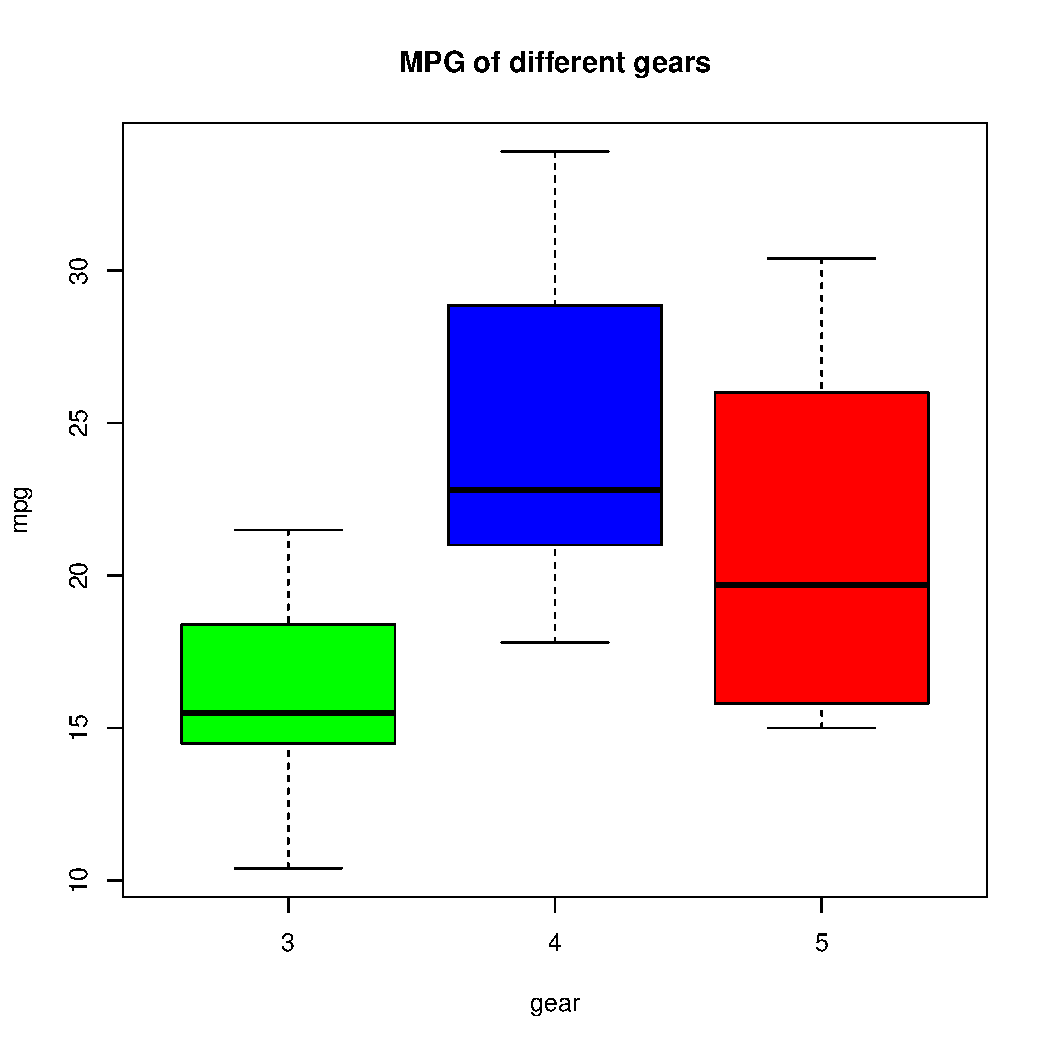
\includegraphics[width=\maxwidth]{figure/Code3_-1} 
\end{knitrout}


\section{Question 3}
Describe the mtcars dataset using tables and graphs. Create a probability distribution table for disp variable.\\

\textbf{Answer}\\
\begin{knitrout}
\definecolor{shadecolor}{rgb}{0.969, 0.969, 0.969}\color{fgcolor}\begin{kframe}
\begin{alltt}
\hlstd{disp_max} \hlkwb{<-} \hlkwd{max}\hlstd{(mtcars}\hlopt{$}\hlstd{disp)}
\hlstd{disp_min} \hlkwb{<-} \hlkwd{min}\hlstd{(mtcars}\hlopt{$}\hlstd{disp)}
\hlstd{bin} \hlkwb{<-} \hlkwd{seq}\hlstd{(disp_min,disp_max,}\hlkwc{by}\hlstd{=}\hlnum{67}\hlstd{)}
\hlstd{disp}\hlkwb{<-}\hlkwd{cut}\hlstd{(mtcars}\hlopt{$}\hlstd{disp,bin)}
\hlstd{freq_table}\hlkwb{<-}\hlkwd{transform}\hlstd{(}\hlkwd{table}\hlstd{(disp))}

\hlkwd{transform}\hlstd{(freq_table,}\hlkwc{Relative_Frequency}\hlstd{=}\hlkwd{prop.table}\hlstd{(Freq),}
          \hlkwc{Probability}\hlstd{=}\hlnum{100}\hlopt{*}\hlkwd{prop.table}\hlstd{(Freq))}
\end{alltt}
\begin{verbatim}
##         disp Freq Relative_Frequency Probability
## 1 (71.1,138]    8         0.28571429   28.571429
## 2  (138,205]    7         0.25000000   25.000000
## 3  (205,272]    2         0.07142857    7.142857
## 4  (272,339]    6         0.21428571   21.428571
## 5  (339,406]    5         0.17857143   17.857143
\end{verbatim}
\end{kframe}
\end{knitrout}

\section{Question 4}
Draw a histogram for the disp variable.\\

\textbf{Answer}\\
\begin{knitrout}
\definecolor{shadecolor}{rgb}{0.969, 0.969, 0.969}\color{fgcolor}\begin{kframe}
\begin{alltt}
\hlkwd{hist}\hlstd{(mtcars}\hlopt{$}\hlstd{disp,}\hlkwc{main}\hlstd{=}\hlstr{"Distribution of disp"}\hlstd{,}\hlkwc{col}\hlstd{=}\hlstr{"purple"}\hlstd{,}\hlkwc{ylim} \hlstd{=} \hlkwd{c}\hlstd{(}\hlnum{0}\hlstd{,}\hlnum{15}\hlstd{),}
     \hlkwc{breaks} \hlstd{=} \hlnum{4}\hlstd{)}
\end{alltt}
\end{kframe}
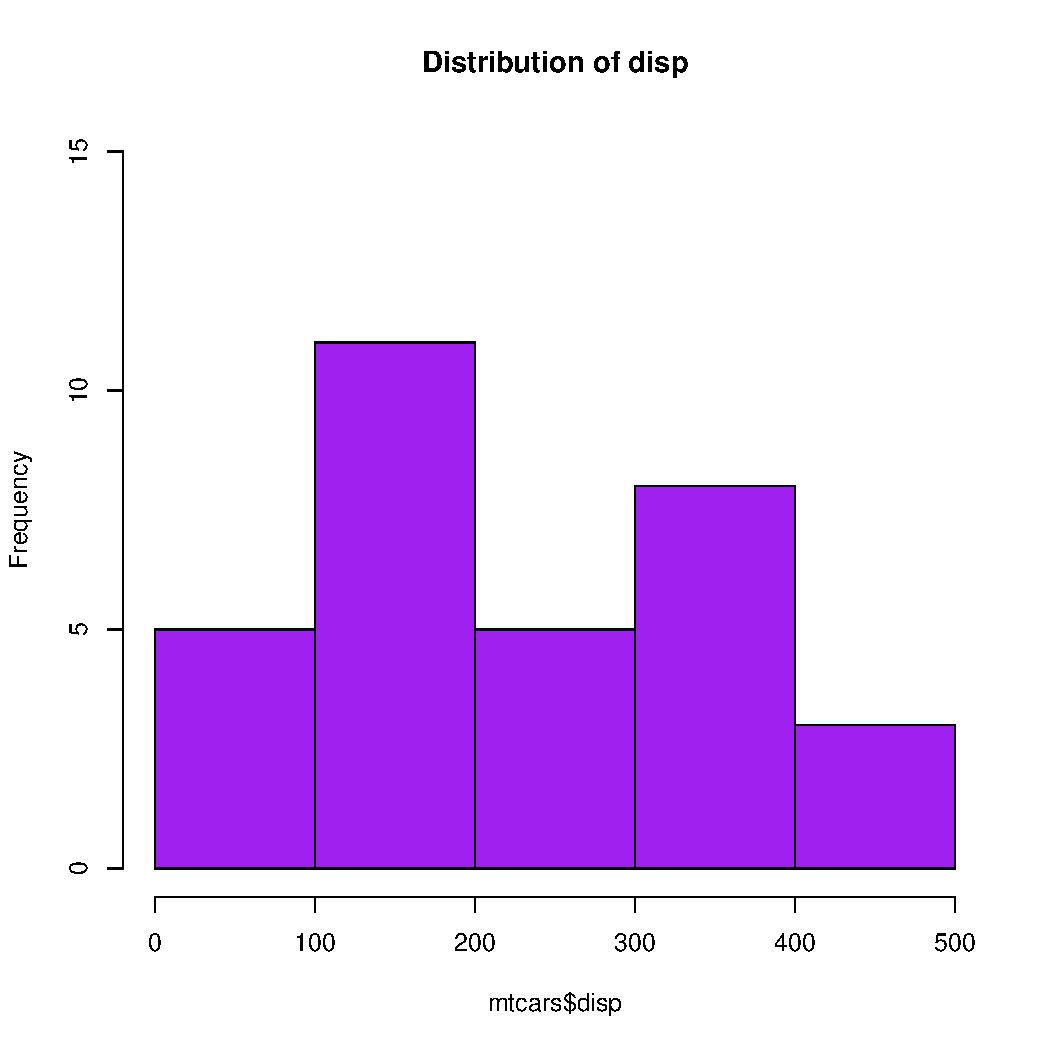
\includegraphics[width=\maxwidth]{figure/Code_1_-1} 
\end{knitrout}

The above histogram shows that the range 100-200 has the highest frequency. 

\section{Question 5}
Draw a piechart for the carb variable.\\

\textbf{Answer}\\
\begin{knitrout}
\definecolor{shadecolor}{rgb}{0.969, 0.969, 0.969}\color{fgcolor}\begin{kframe}
\begin{alltt}
\hlstd{cnt} \hlkwb{<-} \hlkwd{table}\hlstd{(mtcars}\hlopt{$}\hlstd{carb)}
\hlstd{tot} \hlkwb{<-} \hlkwd{sum}\hlstd{(counts)}
\end{alltt}


{\ttfamily\noindent\bfseries\color{errorcolor}{\#\# Error in eval(expr, envir, enclos): object 'counts' not found}}\begin{alltt}
\hlstd{pr} \hlkwb{<-} \hlkwd{round}\hlstd{((cnt}\hlopt{*}\hlnum{100}\hlstd{)}\hlopt{/}\hlstd{tot,}\hlkwc{digits} \hlstd{=} \hlnum{1}\hlstd{)}
\end{alltt}


{\ttfamily\noindent\bfseries\color{errorcolor}{\#\# Error in eval(expr, envir, enclos): object 'tot' not found}}\begin{alltt}
\hlstd{lbls} \hlkwb{<-} \hlkwd{paste}\hlstd{(}\hlkwd{names}\hlstd{(pr),} \hlstr{", "}\hlstd{, pr,} \hlstr{"%"}\hlstd{,} \hlkwc{sep} \hlstd{=} \hlstr{""}\hlstd{)}
\end{alltt}


{\ttfamily\noindent\bfseries\color{errorcolor}{\#\# Error in paste(names(pr), "{}, "{}, pr, "{}\%"{}, sep = "{}"{}): object 'pr' not found}}\begin{alltt}
\hlkwd{pie}\hlstd{(pr,} \hlkwc{labels} \hlstd{= lbls,}
    \hlkwc{main}\hlstd{=}\hlstr{"Pie Chart of Proportion of Cars with Different Number of Carbs"}\hlstd{)}
\end{alltt}


{\ttfamily\noindent\bfseries\color{errorcolor}{\#\# Error in pie(pr, labels = lbls, main = "{}Pie Chart of Proportion of Cars with Different Number of Carbs"{}): object 'pr' not found}}\end{kframe}
\end{knitrout}

The above pie chart shows that the caruretors 2 and 4 have the highest distribution with a percentage of 31.2 %. 

\section{Question 6}
Create a contingency table for gear and carb variables.

\textbf{Answer}\\
The contingeny table for gear and carb variables 

\begin{knitrout}
\definecolor{shadecolor}{rgb}{0.969, 0.969, 0.969}\color{fgcolor}\begin{kframe}
\begin{alltt}
\hlstd{gear_carb_table} \hlkwb{<-} \hlkwd{addmargins}\hlstd{(}\hlkwd{table}\hlstd{(mtcars}\hlopt{$}\hlstd{gear,mtcars}\hlopt{$}\hlstd{carb))}
\hlstd{gear_carb_table}
\end{alltt}
\begin{verbatim}
##      
##        1  2  3  4  6  8 Sum
##   3    3  4  3  5  0  0  15
##   4    4  4  0  4  0  0  12
##   5    0  2  0  1  1  1   5
##   Sum  7 10  3 10  1  1  32
\end{verbatim}
\end{kframe}
\end{knitrout}

This is a contingency table to show the relationship between the variables gear and carb. 

\section{Question 7}
What is the probability when there are 3 gears?

\textbf{Answer}\\
\begin{knitrout}
\definecolor{shadecolor}{rgb}{0.969, 0.969, 0.969}\color{fgcolor}\begin{kframe}
\begin{alltt}
\hlstd{probability_gear_3} \hlkwb{<-}\hlstd{gear_carb_table[}\hlnum{1}\hlstd{,}\hlnum{7}\hlstd{]}\hlopt{/}\hlnum{32}
\end{alltt}
\end{kframe}
\end{knitrout}

The probability when there are 3 gears is 0.46875. The number of observations with 3 gears is 15. Then it is divided by the total number of observations which is 32. 

\section{Question 8}

What is the probability of 3 gears given that there are 2 carbs.\\

\textbf{Answer}\\
\begin{knitrout}
\definecolor{shadecolor}{rgb}{0.969, 0.969, 0.969}\color{fgcolor}\begin{kframe}
\begin{alltt}
\hlstd{probability_gear_3_carb_2} \hlkwb{<-} \hlstd{gear_carb_table[}\hlnum{1}\hlstd{,}\hlnum{2}\hlstd{]}\hlopt{/}\hlnum{32}
\end{alltt}
\end{kframe}
\end{knitrout}

The probability when there are 3 gears and 2 carbs is 0.125. This is because the number of 3 gears and 2 carbs is 4. Then, it is divided by the total number of observations which is 32. 


\section{Question 9}
Proof the Bayesian theorem using the contingency table in Question 6.

\textbf{Answer}\\
\begin{knitrout}
\definecolor{shadecolor}{rgb}{0.969, 0.969, 0.969}\color{fgcolor}\begin{kframe}
\begin{alltt}
\hlstd{probability_carb2} \hlkwb{<-} \hlstd{gear_carb_table[}\hlnum{4}\hlstd{,}\hlnum{2}\hlstd{]} \hlopt{/} \hlnum{32}

\hlstd{probability_gear3_given_carb2} \hlkwb{<-}
  \hlstd{probability_gear_3_carb_2}\hlopt{/}\hlstd{probability_carb2}

\hlstd{probability_carb2_given_gear3} \hlkwb{<-}
  \hlstd{probability_gear_3_carb_2}\hlopt{/}\hlstd{probability_gear_3}
\end{alltt}
\end{kframe}
\end{knitrout}

The probability of gear 3 given 2 carbs is 0.4.

The probability of 2 carbs given gear 3 is 0.2666667.

\begin{knitrout}
\definecolor{shadecolor}{rgb}{0.969, 0.969, 0.969}\color{fgcolor}\begin{kframe}
\begin{alltt}
\hlstd{probability_gear3_given_carb2_2} \hlkwb{<-}
  \hlstd{(probability_carb2_given_gear3}\hlopt{*}\hlstd{probability_gear_3)}\hlopt{/}\hlstd{probability_carb2}
\end{alltt}
\end{kframe}
\end{knitrout}

The answer of the second method of gear 3 given 2 carbs is 0.4.

Hence, the bayesian theorem is proofed. 

\section{Question 10}
Give your solutions in Rnw file, Pdf file and the similarity report.

\section{Marking Scheme}


 
Question 1 = 10\\
Question 2 = 10\\
Question 3 = 10\\
Question 4 = 10\\
Question 5 = 10\\
Question 6 = 10\\
Question 7 = 10\\
Question 8 = 10\\
Question 9 = 10\\
Question 10 = 10\\
Total = 100\\
Mark= 10
